\subsection{Matriz de Capacidade e Saturação (Throughput)}

Embora a arquitetura básica exija escasso poder computacional (sub-100ms com 2 núcleos), a topologia \textit{Medallion} introduz alta complexidade matemática. O carregamento estrito de volumetrias da camada \textit{Silver} (e.g., polígonos GeoJSON de Terras Indígenas) desloca violentamente o gargalo sistêmico do I/O de disco para a CPU e Memória (\textit{Heap} da JVM). Para validar a resiliência estrutural a esse cenário logístico severo, executou-se a matriz de capacidade concorrente.

A avaliação atestou que a renderização de mapas analíticos sob a arquitetura empregada é primariamente \textit{CPU-Bound}. O cenário \textbf{Baseline (1.0 CPU)} apresentou degradação de desempenho logo no primeiro operador, estagnando em \textbf{0,89 QPS} com falha em 42,7\% das requisições (\textit{Timeouts}). Isso atesta que um núcleo solitário não sustenta a alta carga de alocação de memória exigida pelos \textit{Lookups} dimensionais (que transferem as volumosas matrizes GeoJSON, previamente cruzadas na camada Silver pelo Python, para o \textit{Heap} do Druid).

Em contrapartida, a alocação expandida no cenário \textbf{Query Heavy (2.0 CPU)} demonstrou resiliência operacional. O sistema escalou a vazão (\textit{Throughput}) de forma constante, suportando até 16 \textit{threads} simultâneas e formando um platô sustentável na marca de \textbf{\textasciitilde{}2,0 QPS}. Nesse estado resiliente, novas conexões aguardam em fila, mas são integralmente entregues sem geração de \textit{Timeouts HTTP 500} (0\% de erro).

Nota-se, contudo, a presença eventual de \textit{outliers} negativos na curvatura de vazão linear. Em pontos específicos da escalada da carga, o sistema sofreu quedas abruptas de vazão em janelas milissegundares. Levanta-se a forte hipótese técnica de que este comportamento anômalo remeta a pausas prolongadas de \textit{Garbage Collection} (GC \textit{Stop-The-World}) e a eventos de \textit{Thread Contention}, embora essa suposição exigisse medições com \textit{profilers} ativos na JVM para constatação isolada.

\begin{figure}[H]
    \centering
    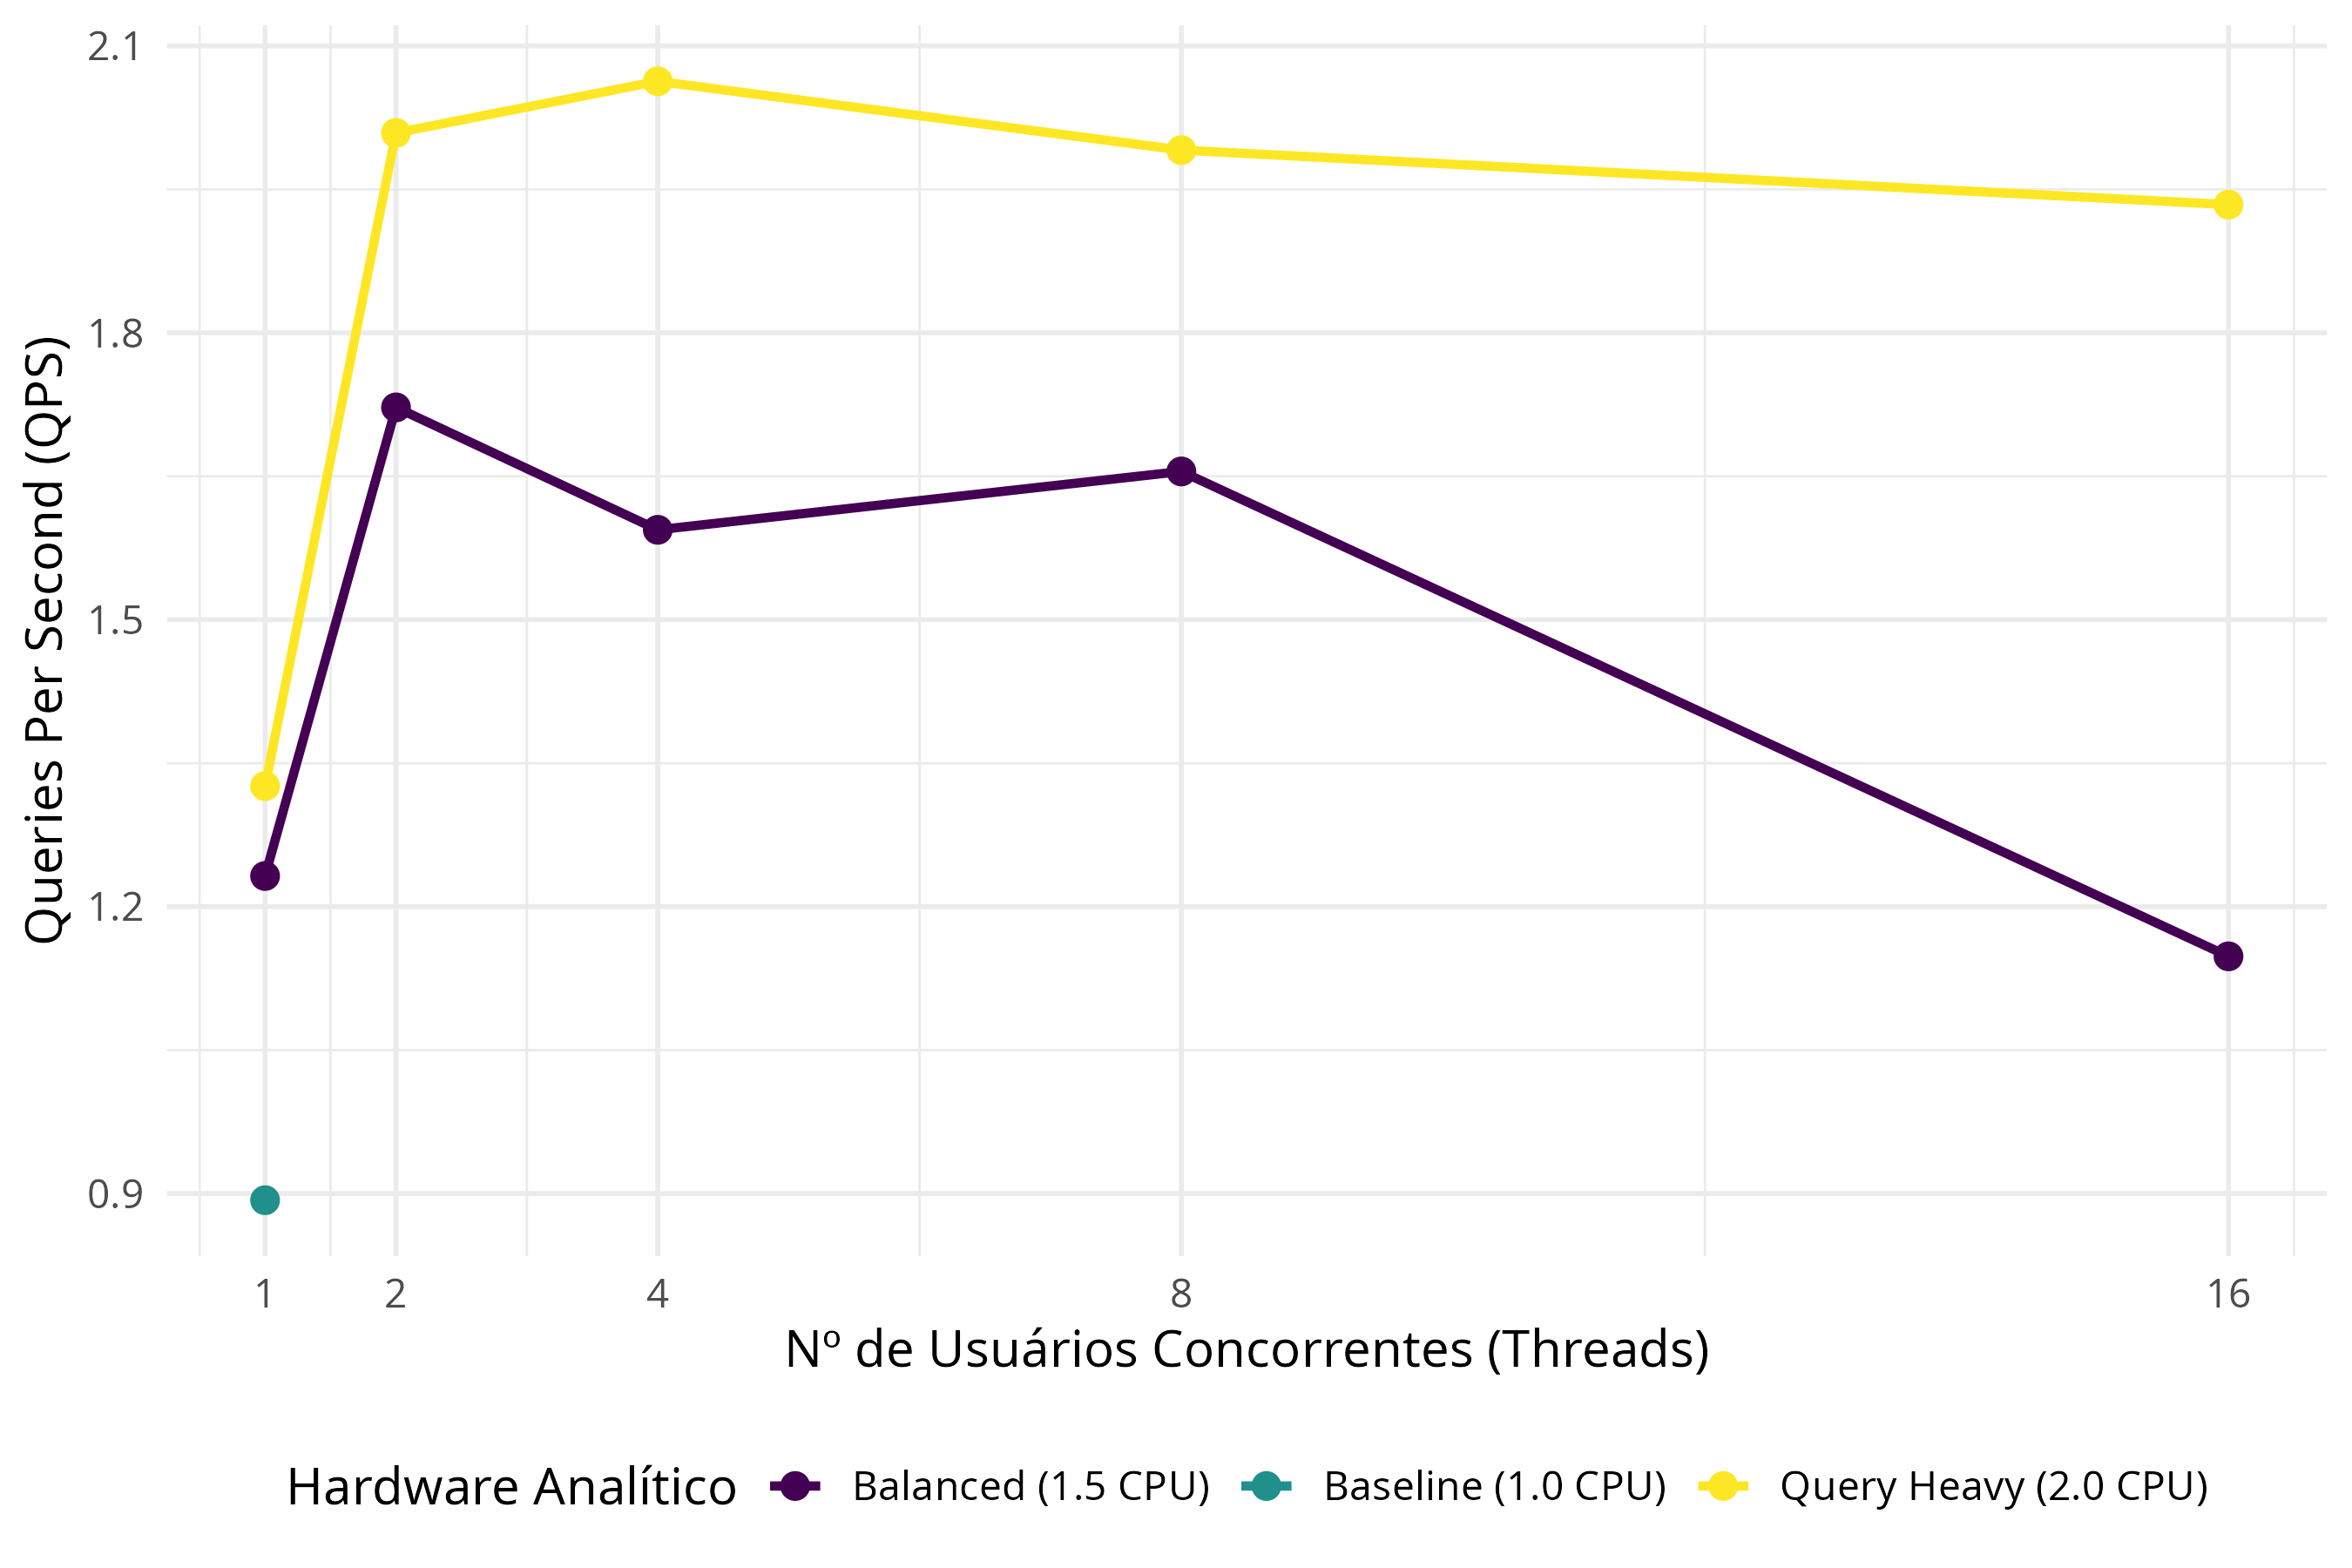
\includegraphics[width=0.8\textwidth]{analise_R/plots/qps_saturation_new.png}
    \caption{Vazão Analítica (QPS) por Perfil de Escalabilidade.}
    \label{fig:qps_saturation}
\end{figure}

\subsection{Explosão de Latência e Percentil 95 (P95)}

Conforme demonstrado estatisticamente, no cenário \textit{Baseline} a latência e o volume de falhas descontrolaram-se já no primeiro operador em rede. Em contraste, o cenário \textit{Query Heavy} absorveu o impacto geométrico sem gerar interrupções, contendo a latência P95 na faixa aceitável de \textbf{\textasciitilde{}2,8 segundos} (com 2 operadores) até o limiar de \textbf{\textasciitilde{}8,2 segundos} sob o estresse de 8 operadores processando agregações massivas simultaneamente.

Contudo, fora da curva de 95\% (\textit{outliers}), registraram-se picos de latência. Esses engasgos ocorrem quando cruzamentos espaciais densos (e.g., sobreposição espacial em Terras Indígenas) esgotam a memória \textit{Heap} da JVM e os \textit{Merge Buffers}, forçando pausas prolongadas de \textit{Garbage Collection} (GC). Ressalta-se que tais anomalias foram induzidas por \textit{queries} puramente de estresse (sem amarras temporais). Na operação real do SIRDA, filtros de temporalidade (ex: janela crítica de 7 dias) impedem que um pacote GeoJSON dessa magnitude congestione a memória em uma única requisição.

\begin{figure}[H]
    \centering
    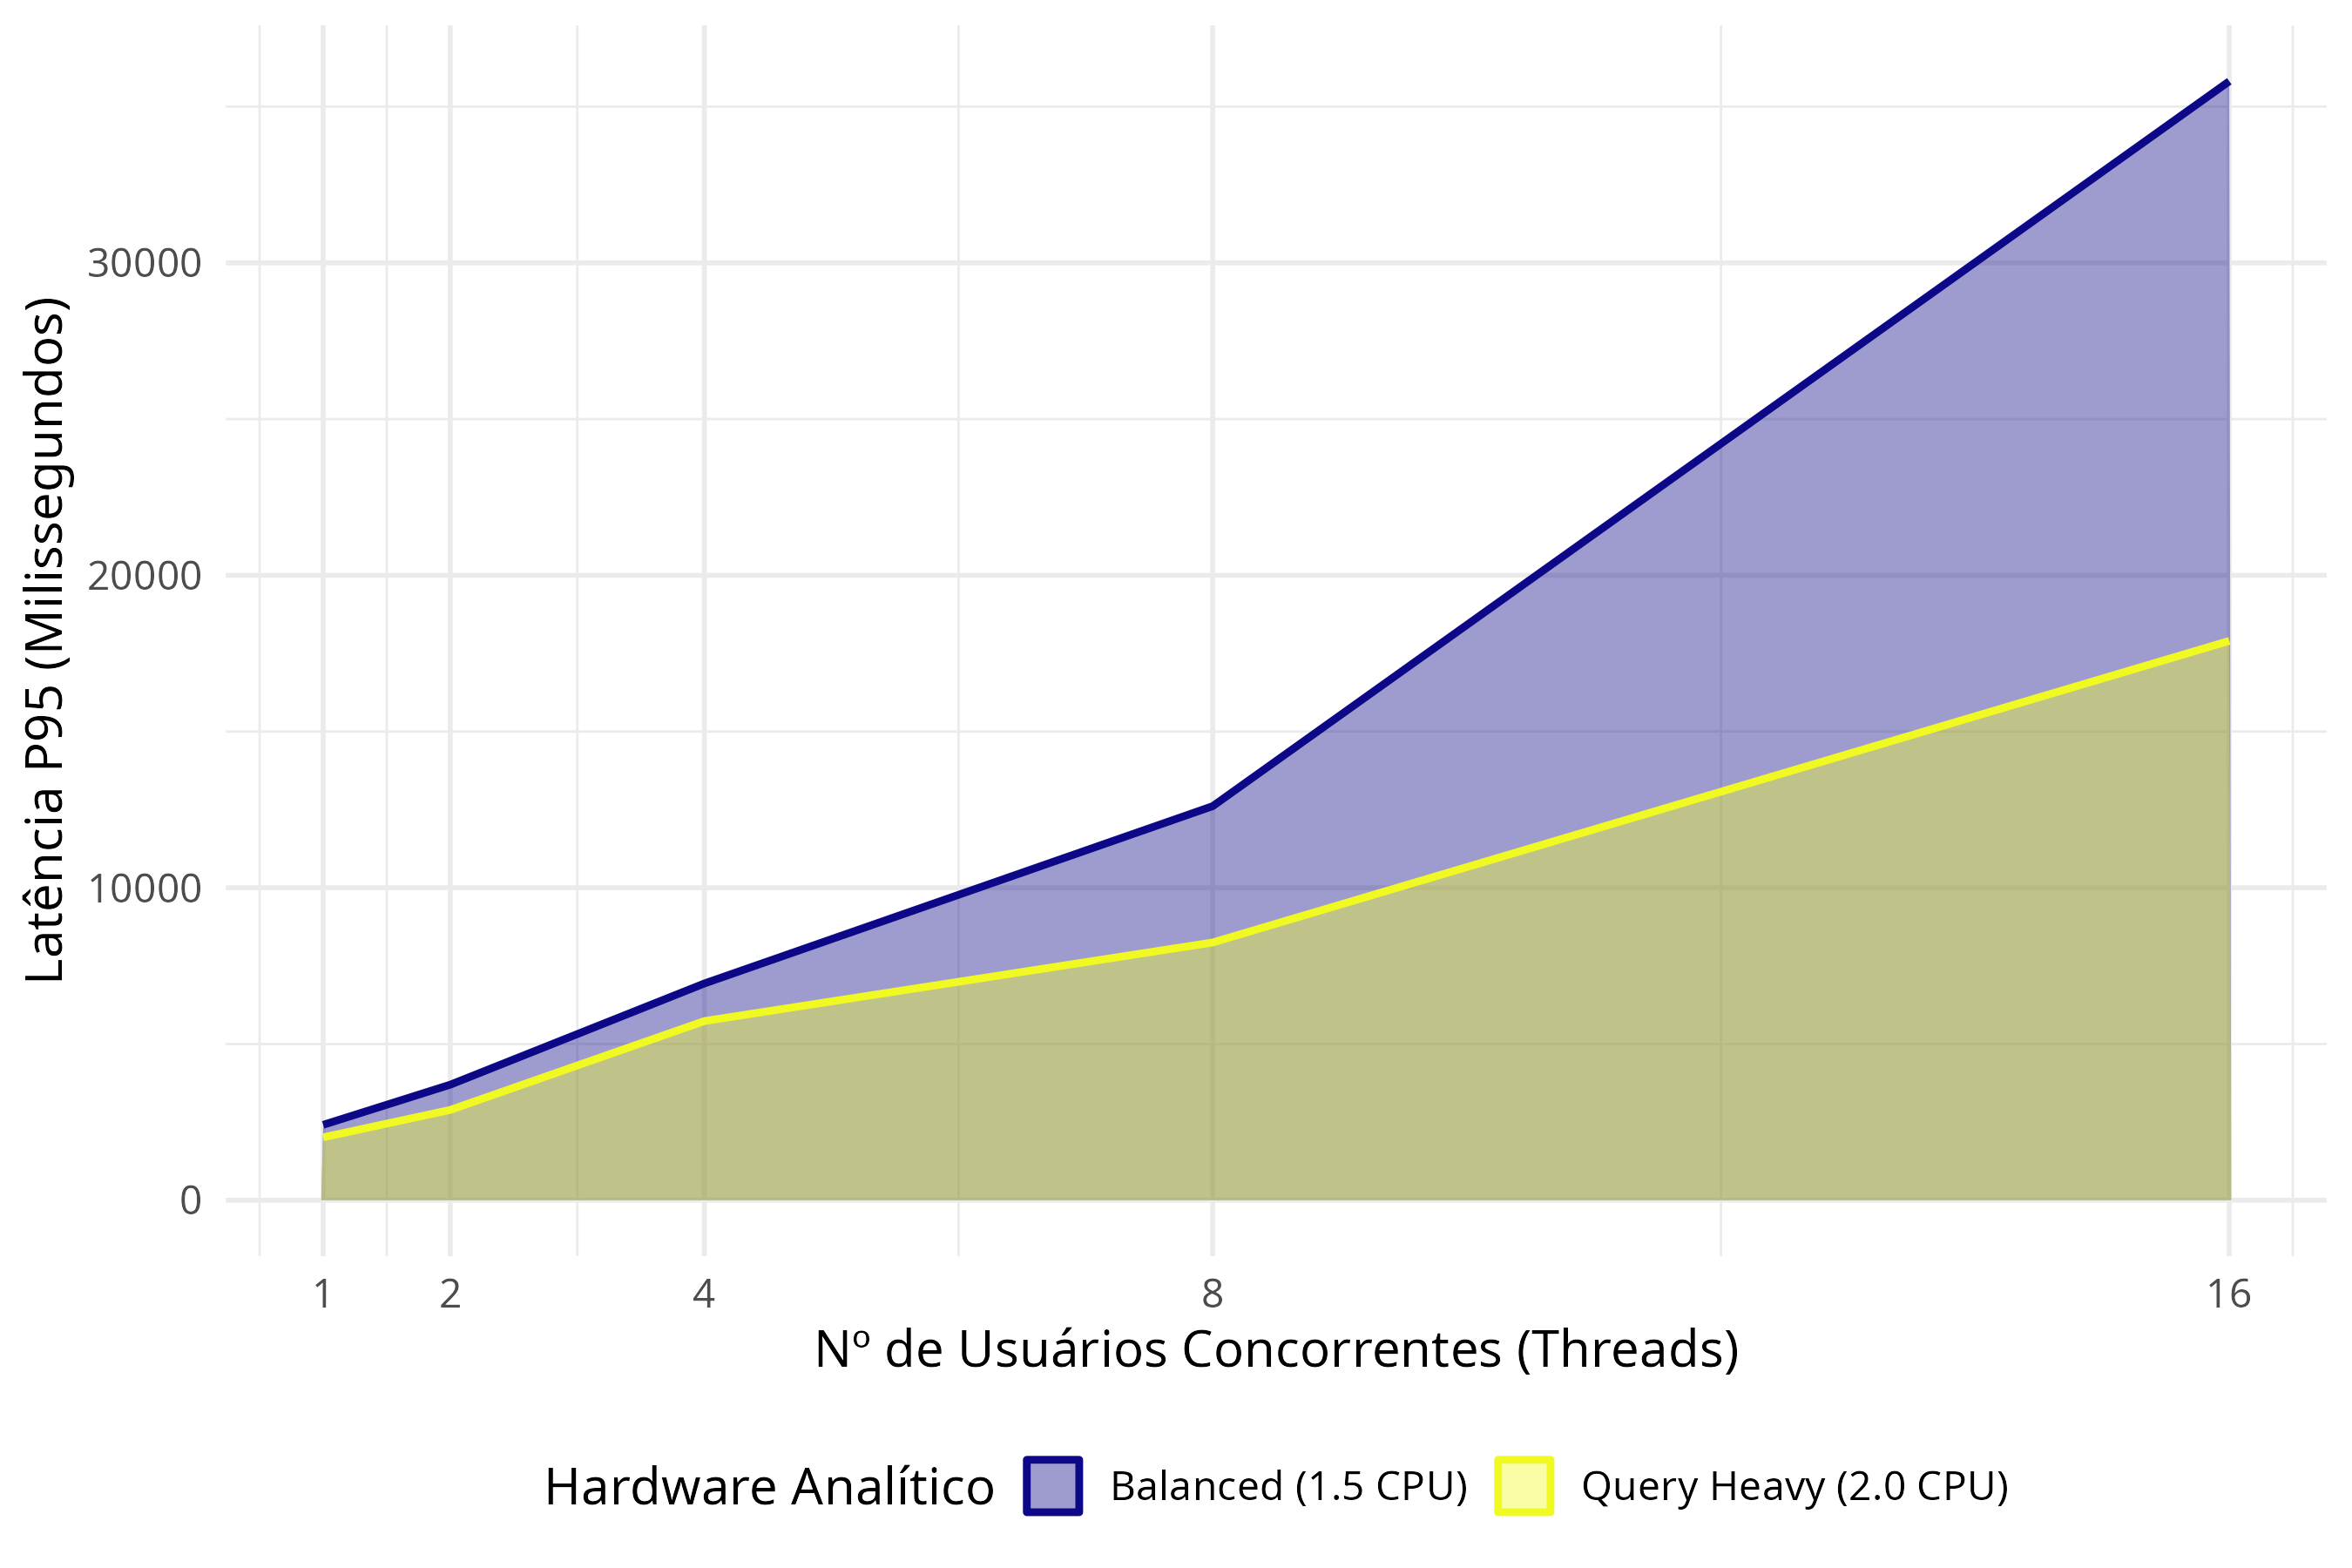
\includegraphics[width=0.8\textwidth]{analise_R/plots/p95_latency_new.png}
    \caption{Degradação de Latência (P95) durante Escalonamento.}
    \label{fig:p95_latency}
\end{figure}
